
\section{Introduction}

Introductory part specifying topic and context of the student project. It
should briefly lay out what you are going to show in the project report. This
is somewhat like a preview for the reader. 
To better link the project to the existing research literature, a brief summary
of the original research article that was used as the starting point for the
student project can be included.
This brief summary should detail the topic of the article, the motivation of the
presented study, and a list of the central findings of the article. 
Include about 30 references to support your report. Here you can find examples
of how to format references to research articles \cite{Akhmediev:PRA:1995},
books \cite{Drazin:book:1989}, or other online media \cite{Scipy}.

\section{Methods}

\subsection{Mathematical model}
Detail the computational problem studied in your student project. E.g., if 
you study the nonlinear Schr\"odinger equation you might start like this:\\

\noindent The computational problem studied in this student project is an initial
value problem with periodic boundary conditions, consisting of the propagation
of a complex-valued field $A(z,t)$ along the propagation coordinate $z$ on a
periodic $t$-domain of extend $T$, subject to the nonlinear Schr\"odinger equation (NSE) 
\begin{align}
\begin{cases}
\partial_z A(z,t) =-\frac{i}{2}\beta_2 \partial_t^2 A(z,t) + i\gamma |A(z,t)|^2 A(z,t) , & \quad z\geq0,~-T/2\leq t\leq T/2,\label{eq:NSE}\\
A(z,-T/2)=A(z,T/2), &\quad z\geq 0,\\
A(z,t)|_{z=0} = A_0(t), &\quad -T/2\leq t \leq T/2.
\end{cases}
\end{align}
The field $A(z,t)$ describes the complex envelope of an optical pulse and
Eq.~(\ref{eq:NSE}) models its $z$-propagation 
through a single-mode fiber governed by the group-velocity
dispersion (GVD) parameter $\beta_2$, and the nonlinear parameter $\gamma$.
The pulse dynamics is resolved in a frame of reference moving with the
group velocity of the pulse.

\subsection{Numerical method}
Review numerical methods that are available to solve for the computational
problem.  Detail the numerical method you used to study the computational
problem.

\subsection{Implementation}
If you like, elaborate on aspects of your implementation. An example of how to
display a code-snippet is illustrated in code-listing \ref{lst:NSE}. In
particular, if you use a software development platform such as GitHub to host
your developed code, you can point out and advertise that here.
For a guide on how to structure your computational project, see Ref.~\cite{Noble:PLOS:2009}.

% BEGIN - LISTING %%%%%%%%%%%%%%%%%%%%%%%%%%%%%%%%%%%%%%%%%%%%%%%%%%%%%%%%%%%%%%%%%%%%%
\begin{lstlisting}[
caption={Python function implementing a split-step Fourier method 
for solving the nonlinear Schr\"odinger equation.}, 
label=lst:NSE]
def NSE_SSFM_simple(z, t, A0_t, beta2, gamma, nSkip):
    """Split step Fourier method using simple operator splitting

    Implements divide-and-conquer strategy to solve the nonlinear
    Schroedinger equation (NSE). Pulse propagation is performed
    using a simple splitting scheme.

    NOTES:
        - uses abbreviations FT, specifying the DFT, and IFT, 
          specifying its inverse. These are defined at the 
          beginning of the script right beneath the imports.

    Args:
        z (array): samples along propagation distance
        t (array): time samples
        A0_t (array): time domain field envelope
        beta2 (float): 2nd order dispersion parameter
        gamma (float): nonlinear parameter
        nSkip (int): keep only each nSkip-th field configuration

    Returns: (z,Azt)
        z (array): z-samples at which field envelope is recorded
        Azt (array): resulting time domain field envelope
    """
    # -- convenient abbreviations
    dz = z[1]-z[0]
    dt = t[1]-t[0]
    # -- work arrays and data structures for results
    A_t  = np.copy(A0_t)
    w = nfft.fftfreq(t.size,d=dt)*2*np.pi
    res_z = []; res_z.append(0)
    res_A = []; res_A.append(A0_t)

    for idx in range(1, z.size):
        # -- nonlinear sub-step
        A_t =  A_t*np.exp(1j*gamma*np.abs(A_t)**2*dz)
        # -- linear sub-step
        A_t =  IFT(np.exp(0.5j*beta2*w*w*dz)*FT(A_t))
        # -- store intermediate results
        if idx%nSkip==0:
            res_z.append(z[idx])
            res_A.append(A_t)

    return np.asarray(res_z), np.asarray(res_A)
\end{lstlisting}
% END - LISTING %%%%%%%%%%%%%%%%%%%%%%%%%%%%%%%%%%%%%%%%%%%%%%%%%%%%%%%%%%%%%%%%%%%%%



\section{Results}

Summarize the numerical experiments carried out during your student project.
Include figures like Fig.~\ref{fig:fig01} to illustrate your findings.  For a
guide on publication ready scientific figures, see
Ref.~\cite{Rougier:PLOS:2014}.  Take care to include enough detail so that
someone reading your report is able to reproduce the results.  Use subsections
to structure your results in a meaningful way.

% BEGIN - FIGURE %%%%%%%%%%%%%%%%%%%%%%%%%%%%%%%%%%%%%%%%%%%%%%%%%%%%%%%%%%%%%%%%%%%%%
\begin{figure}[b!]
\centering
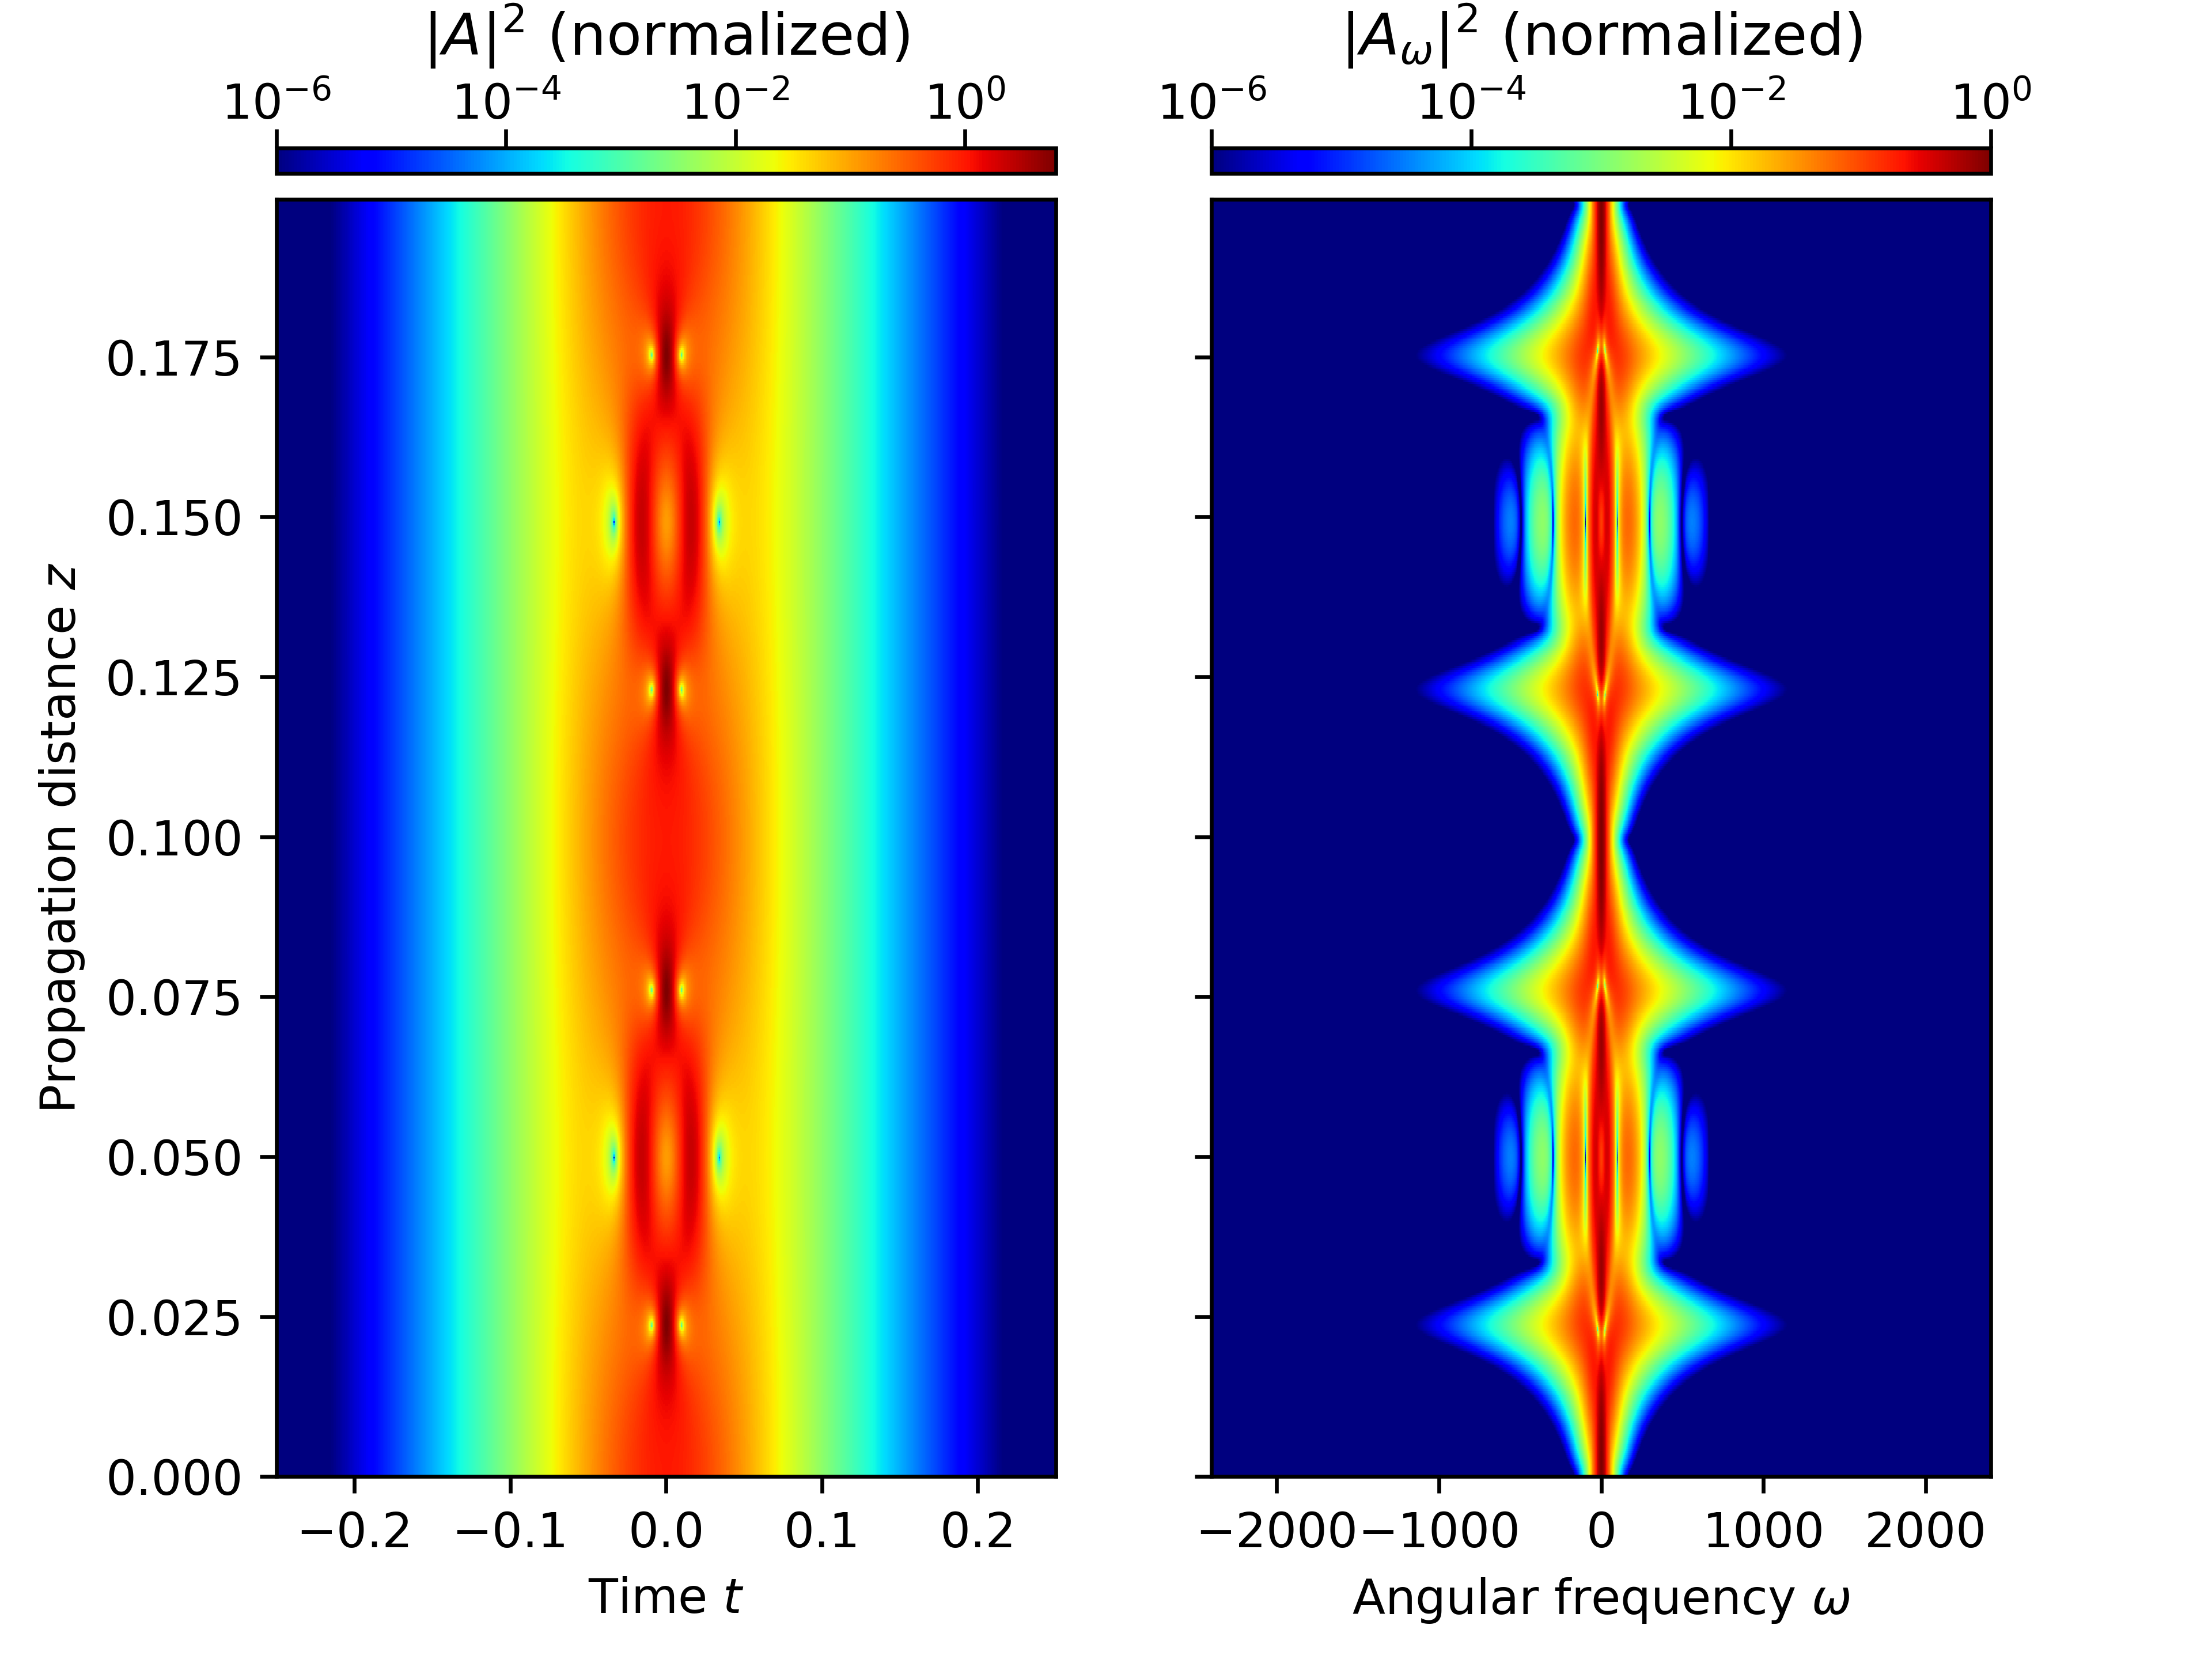
\includegraphics[width=\linewidth]{./figure01.png}
\caption{
Evolution of the intensity (left) and spectral intensity (right) for a 
soliton of order $N=3$ governed by Eq.~(\ref{eq:NSE}).}
\label{fig:fig01}
\end{figure}
% END - FIGURE %%%%%%%%%%%%%%%%%%%%%%%%%%%%%%%%%%%%%%%%%%%%%%%%%%%%%%%%%%%%%%%%%%%%%


\section{Discussion \& Summary}

Give a brief summary of what you did during your student project. This should
also include the main results you obtained in the course of your project work.

